%----------------------------------------------------------------------------------------
%	CHAPTER 4
%----------------------------------------------------------------------------------------
\chapterimage{ChapterImages/chapter4.png} % Chapter heading image

\chapter{Working with Text Files in Linux}
\label{ch:textfiles}

In Linux, text files form the foundation of nearly every system operation. Configuration files, shell scripts, system logs, and most forms of data are stored as plain text. Therefore, the ability to view, edit, search, and process text files efficiently is an essential skill for any Linux user or system administrator.

This chapter introduces the common command-line tools used to interact with text files: how to read file contents, modify text data, search using patterns, and process text using filters and redirection.

\section{Viewing Text Files}
To inspect file contents, Linux provides multiple commands suited for different purposes:

\begin{itemize}
    \item \texttt{cat} -- displays the entire content of a file:
\begin{lstlisting}[language=Terminal]
$ cat <file>
\end{lstlisting}

    \item \texttt{less} / \texttt{more} -- display large files one screen at a time, letting you scroll through the file (press \texttt{q} to quit):
\begin{lstlisting}[language=Terminal]
$ less <file>
$ more <file>
\end{lstlisting}
    \texttt{less} is the more modern of the two -- it lets you scroll both forward and backward and doesn't need to load the whole file up front, so prefer it over \texttt{more} when both are available.

    \item \texttt{head} -- shows the first 10 lines of a file:
\begin{lstlisting}[language=Terminal]
$ head -n 10 <file>
\end{lstlisting}

    \item \texttt{tail} -- shows the last 10 lines of a file:
\begin{lstlisting}[language=Terminal]
$ tail -n 10 <file>
\end{lstlisting}

    \item \texttt{tail -f} -- continuously monitors a file for new lines as they are written, without exiting; ideal for watching a log file in real time:
\begin{lstlisting}[language=Terminal]
$ tail -f <logfile>
\end{lstlisting}
\end{itemize}

\section{Editing Text Files}
Linux provides several text editors that can be used directly from the terminal or through a graphical interface. Each editor offers a different balance of simplicity and power.

Some important text editors are:
\begin{itemize}
    \item \texttt{nano}: a simple, beginner-friendly terminal-based editor.
    \item \texttt{vim}: a powerful modal editor for advanced users.
    \item \texttt{gedit}: a graphical text editor suitable for desktop environments.
\end{itemize}
\textbf{Note:} Editing system files may require administrative privileges; use \texttt{sudo} if necessary.

\textbf{Opening an Editor}\\
To open a file for editing, use the editor's command followed by the filename:
\begin{lstlisting}[language=Terminal]
$ nano filename.txt
$ vim filename.txt
$ gedit filename.txt
\end{lstlisting}
If the file does not exist, it is created automatically when you save and exit.

\subsection{Using Nano}
\texttt{nano} is a simple and beginner-friendly terminal text editor.

\textbf{To start:}
\begin{lstlisting}[language=Terminal]
$ nano filename.txt
\end{lstlisting}

\textbf{Basic Commands} (shown at the bottom of the screen):
\begin{itemize}
    \item \texttt{Ctrl + O} --- Save the file (then press Enter to confirm).
    \item \texttt{Ctrl + X} --- Exit the editor.
    \item \texttt{Ctrl + K} --- Cut a line.
    \item \texttt{Ctrl + U} --- Paste the cut line.
    \item \texttt{Ctrl + W} --- Search for text.
    \item \texttt{Ctrl + G} --- Display help.
\end{itemize}
\texttt{nano} is ideal for quick edits and configuration file changes.

\subsection{Using Vim}
\texttt{vim} is a powerful modal text editor designed for advanced editing and automation tasks.

\textbf{To start:}
\begin{lstlisting}[language=Terminal]
$ vim filename.txt
\end{lstlisting}

\textbf{Modes:}
\begin{itemize}
    \item \textbf{Normal mode} --- used for navigation and commands.
    \item \textbf{Insert mode} --- used for typing text.
    \item \textbf{Command mode} --- used for saving and quitting.
\end{itemize}

\textbf{Basic Commands:}
\begin{itemize}
    \item Press \texttt{i} --- enter Insert Mode to start editing.
    \item Press \texttt{Esc} --- return to Normal Mode.
    \item Type \texttt{:w} --- save the file.
    \item Type \texttt{:q} --- quit Vim.
    \item Type \texttt{:wq} --- save and quit.
    \item Type \texttt{:q!} --- quit without saving.
\end{itemize}
\texttt{vim} is efficient for editing large files, programming, and automating repetitive edits.

\subsection{Using Gedit}
\texttt{gedit} is a graphical text editor suitable for desktop environments such as Ubuntu.

\textbf{To start (GUI mode):}
\begin{lstlisting}[language=Terminal]
$ gedit filename.txt &
\end{lstlisting}
The trailing \texttt{\&} runs \texttt{gedit} in the background, so the terminal remains usable while the editor stays open.

\textbf{Basic Features:}
\begin{itemize}
    \item Menu-based options for opening, saving, and editing files.
    \item Syntax highlighting for many programming languages.
    \item Ideal for users who prefer a graphical interface.
\end{itemize}

\section{Searching in Files}
Searching for specific content within text files is a common and powerful operation in Linux. The main tool for this purpose is \texttt{grep} (Global Regular Expression Print). It prints lines that match a given pattern or word, making it especially useful for analyzing log files, configuration files, and source code.

\subsection{Basic Usage}
The simplest form of the \texttt{grep} command searches for a specific word or phrase:
\begin{lstlisting}[language=Terminal]
$ grep "pattern" filename.txt
\end{lstlisting}
This command prints all lines in \texttt{filename.txt} that contain the word \texttt{pattern}.

\textbf{Example:}
\begin{lstlisting}[language=Terminal]
$ grep "error" system.log
\end{lstlisting}
This displays all lines in \texttt{system.log} that contain the word ``\texttt{error}''.

\subsection{Common Options}
\texttt{grep} supports several useful options that enhance its searching capabilities:
\begin{table}[h!]
\centering
\small
\renewcommand{\arraystretch}{1.3}
\begin{tabular}{|>{\centering\arraybackslash}p{2cm}|>{\raggedright\arraybackslash}p{6cm}|>{\raggedright\arraybackslash}p{6cm}|}
\hline
\textbf{Option} & \textbf{Description} & \textbf{Example} \\ \hline
\texttt{-i} & Ignore case differences when searching & \texttt{grep -i "error" log.txt} \\ \hline
\texttt{-n} & Display line numbers along with matches & \texttt{grep -n "root" /etc/passwd} \\ \hline
\texttt{-v} & Invert match (show lines that \emph{do not} contain the pattern) & \texttt{grep -v "INFO" logfile.txt} \\ \hline
\texttt{-r} & Search recursively through all subdirectories & \texttt{grep -r "main" ./src} \\ \hline
\texttt{-A N} & Show \texttt{N} lines \emph{after} each match & \texttt{grep -A 2 "ERROR" log.txt} \\ \hline
\texttt{-B N} & Show \texttt{N} lines \emph{before} each match & \texttt{grep -B 2 "ERROR" log.txt} \\ \hline
\texttt{-C N} & Show \texttt{N} lines of context (before and after matches) & \texttt{grep -C 3 "ERROR" log.txt} \\ \hline
\end{tabular}
\caption{Common \texttt{grep} Command Options in Linux}
\label{tab:grep-options}
\end{table}

\textbf{Searching Multiple Files:}\\
You can search across several files at once:
\begin{lstlisting}[language=Terminal]
$ grep "main" *.c
\end{lstlisting}
This command finds occurrences of ``\texttt{main}'' in all \texttt{.c} files in the current directory.

\subsection{Using Regular Expressions with Grep}
\texttt{grep} can use regular expressions (regex) to match complex patterns instead of exact words.

\textbf{Examples:}
\begin{lstlisting}[language=Terminal]
$ grep "^A" names.txt        # Lines starting with A
$ grep "error$" log.txt      # Lines ending with 'error'
$ grep "[0-9]" data.txt      # Lines containing a number
$ grep -E "cat|dog" pets.txt # Lines containing 'cat' or 'dog'
\end{lstlisting}
Use \texttt{grep -E} (or \texttt{egrep}) for extended regular expressions, which support more advanced patterns such as alternation (\texttt{|}).

\section{Text Processing Commands}
Linux provides several commands for handling and analyzing text files. These commands are often used together to \textbf{filter}, \textbf{modify}, or \textbf{summarize} data.

\textbf{Common Text Processing Commands:}
\begin{itemize}
    \item \texttt{cut} -- extract specific columns or fields from a file.
\begin{lstlisting}[language=Terminal]
$ cut -d ":" -f1 /etc/passwd    # Shows the first field in each line
\end{lstlisting}

    \item \texttt{tr} -- translate or delete characters.
\begin{lstlisting}[language=Terminal]
$ tr 'a-z' 'A-Z' < file.txt    # Converts all letters to uppercase
\end{lstlisting}

    \item \texttt{sort} -- sort lines alphabetically or numerically.
\begin{lstlisting}[language=Terminal]
$ sort names.txt
\end{lstlisting}

    \item \texttt{uniq} -- remove duplicate lines (usually used after \texttt{sort}).
\begin{lstlisting}[language=Terminal]
$ sort names.txt | uniq
\end{lstlisting}

    \item \texttt{wc} -- count lines, words, and characters.
\begin{lstlisting}[language=Terminal]
$ wc -l file.txt
\end{lstlisting}

    \item \texttt{awk} -- print selected columns or perform basic text processing.
\begin{lstlisting}[language=Terminal]
$ awk '{print $1, $3}' data.txt
\end{lstlisting}

    \item \texttt{sed} -- search and replace text.
\begin{lstlisting}[language=Terminal]
$ sed 's/error/warning/g' logfile.txt
\end{lstlisting}
\end{itemize}

These commands can be combined with pipes (\texttt{|}) for more powerful results.\\
\textbf{Example:}
\begin{lstlisting}[language=Terminal]
$ cat logfile.txt | grep "ERROR" | sort | uniq -c
\end{lstlisting}
This finds all ``\texttt{ERROR}'' lines, sorts them, removes duplicates, and counts occurrences.

\section{Redirection and Pipes}
Redirection and pipes let you control where a command's input and output go. They are essential for saving results and combining commands. Figure~\ref{fig:redirection-pipes} summarizes the three mechanisms below.

\begin{figure}[h]
    \centering
    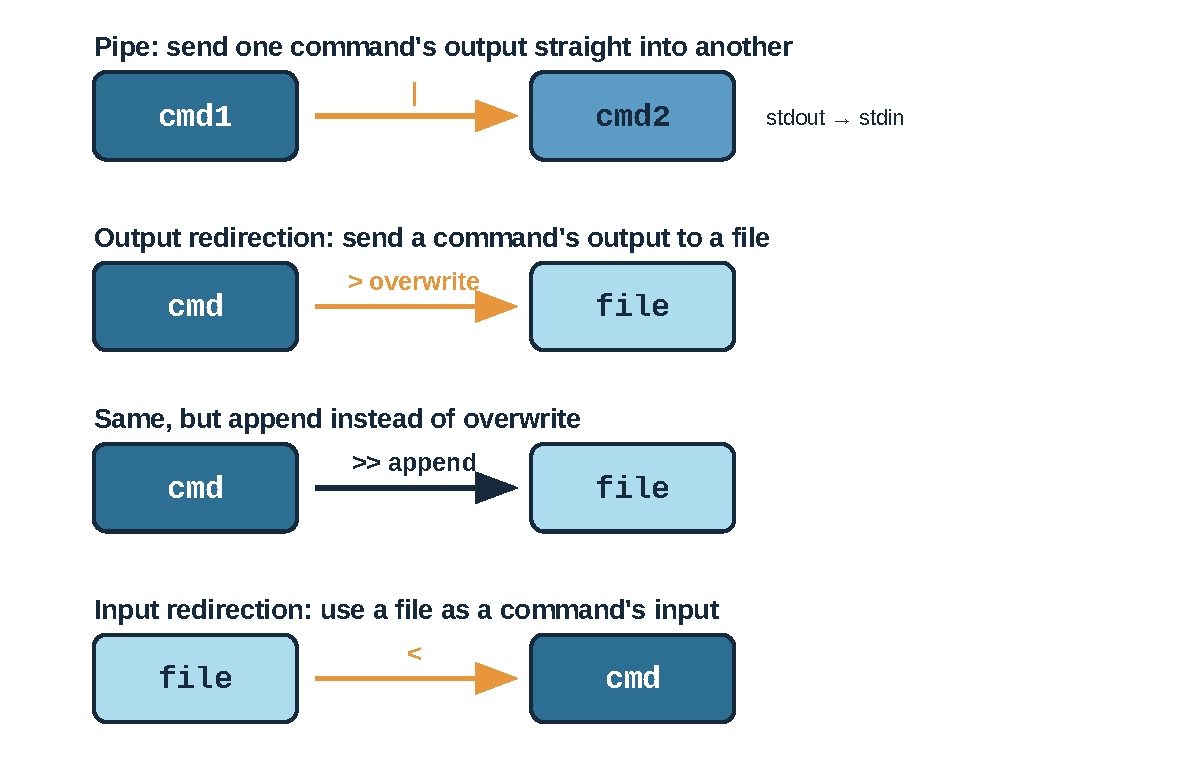
\includegraphics[width=0.9\textwidth]{Images/Chapter4/redirection-pipes.pdf}
    \caption{Output redirection, append, input redirection, and pipes: where data goes in each case.}
    \label{fig:redirection-pipes}
\end{figure}

\subsection{Output Redirection}
\begin{itemize}
    \item \texttt{>} --- write output to a file, overwriting it:
\begin{lstlisting}[language=Terminal]
$ echo "Hello" > greeting.txt
\end{lstlisting}
    \item \texttt{>>} --- append output to a file:
\begin{lstlisting}[language=Terminal]
$ echo "World" >> greeting.txt
\end{lstlisting}
\end{itemize}

\subsection{Input Redirection}
\begin{itemize}
    \item \texttt{<} --- use a file as input instead of the keyboard:
\begin{lstlisting}[language=Terminal]
$ sort < names.txt
\end{lstlisting}
\end{itemize}

\subsection{Pipes}
\begin{itemize}
    \item \texttt{|} --- send the output of one command to another:
\begin{lstlisting}[language=Terminal]
$ cat file.txt | grep "error"
$ ps aux | grep "python"
\end{lstlisting}
\end{itemize}

\textbf{Example:}
\begin{lstlisting}[language=Terminal]
$ grep "ERROR" log.txt | sort | uniq -c > result.txt
\end{lstlisting}
\textbf{This command:}
\begin{itemize}
    \item Finds lines with ``\texttt{ERROR}''
    \item Sorts and counts them
    \item Saves the output to \texttt{result.txt}
\end{itemize}
